\section{Softwarearchitektur}

\subsection{Strategie}

\subsection{Erkundung und Speicherung der Karte} \label{erkundungDerKarte}

\begin{figure}[h]
    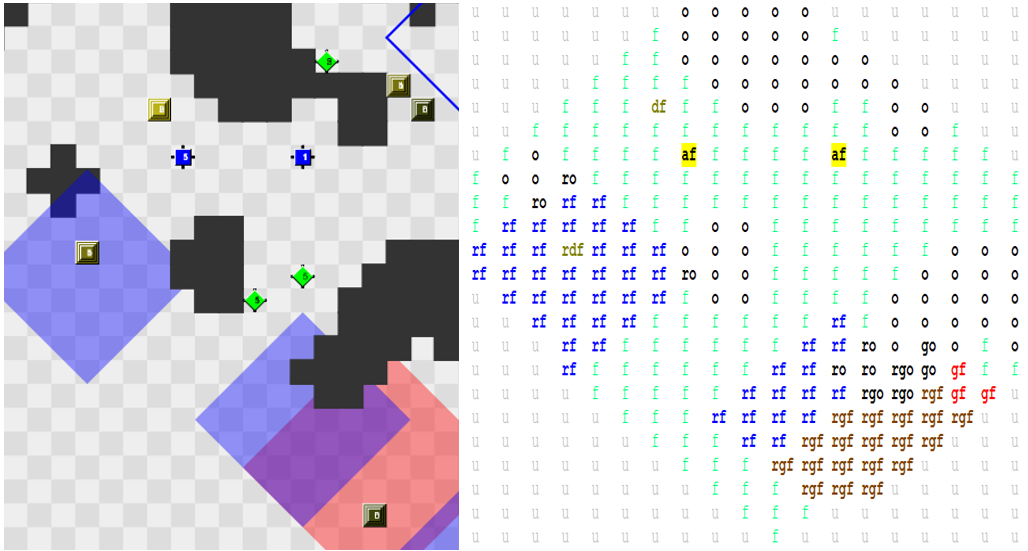
\includegraphics[width=1.0\textwidth]{./Abbildungen/map.png}
    \centering
    \caption{Links: Screenshot der Karte, Rechts: \NextMap-Objekt einer Gruppe mit 2 Agents als Output in eine .txt-Datei. \newline Legende: \underline{a}gent, \underline{d}ispenser, \underline{f}ree, \underline{g}oal zones, \underline{o}bstacles, \underline{r}ole zones, \underline{u}nknown}
\end{figure}

In jedem Schritt eines Spiels kann über die \Percepts abgerufen werden, welche Objekte für einen \Agent aktuell sichtbar sind. Wie weit ein \Agent sehen kann, hängt von der Rolle ab und wird basierend auf der Manhattan-Distanz berechnet. Die von einem \Agent wahrgenommenen \Things werden hierbei mit relativer Distanz zur Position des \Agents angegeben. Wenn sich beispielsweise ein \Obstacle zwei Felder rechts neben dem \Agent befindet, wird dieses im \Percept mit den Koordinaten [2, 0] angegeben. Bewegt sich der \Agent um ein Feld nach rechts, wird das \Obstacle dann im Abstand [1, 0] gesehen. Informationen vergangener \Percepts sind nicht verfügbar, d.h. ein \Agent besitzt zunächst einmal kein „Gedächtnis“. Um eine zielgerichtete Planung der \Agents umzusetzen, ist es daher erforderlich, die in jedem \Step wahrgenommenen Sichten zu speichern und so Schritt-für-Schritt eine Karte aufzubauen. Es ergeben sich folgende Anforderungen:
\begin{enumerate}
\item Jeder \Agent soll die in den einzelnen \Steps wahrgenommenen Dinge speichern und auf diese zu einem späteren Zeitpunkt zugreifen können. 
\item Da manche Informationen der Karte dynamisch sind (z.B. können \Obstacles per \textit{clear()} entfernt werden), ist auch eine Aktualisierung bereits gespeicherter Positionen erforderlich. 
\item \Agents sollten bestenfalls dieselbe Karte verwenden, sodass jeder \Agent aus der Erkundung / aus dem Wissen der anderen \Agents schöpfen kann.
\item Üblicherweise werden die Spiele mit einer sich wiederholenden Karte mit unbekannter Kartengröße gespielt. Um eine effiziente Planung zu ermöglichen, sollen die Kartengröße ermittelt und die Wiederholungen bei Speicherung der Karte berücksichtigt werden.
\end{enumerate}

\subsubsection{Implementierung} ~\\
Es wurden im Wesentlichen folgende Klassen zur Umsetzung implementiert:
\begin{itemize}
\item \NextMapTile: Beschreibung eines einzelnen Feldes mit den Eigenschaften Position, Typ und \Step (Schritt, wann die Position zuletzt gesehen wurde).   
\item \NextMap: Beschreibung der Karte als Ganzes durch Speicherung der wahrgenommenen \Things je \Step als \NextMapTiles. Um eine Mehrfach-Belegung einer Position zu ermöglichen (z.B. \GoalZone und \Obstacle auf derselben Position), werden die verschiedenen Typen in jeweils eigenen Datenstrukturen gespeichert (Karte der \Obstacles, Karte der \GoalZones, etc.).
\item \NextGroup: Gruppierung von 1…n \Agents, welche dieselbe Karte nutzen. Jede Gruppe enthält genau ein \NextMap-Objekt. 
\end{itemize}

\subsubsection{Aktualisierung} ~\\
Je \Agent wird geprüft, ob im letzten \Step ein erfolgreicher \move-Befehl ausgeführt wurde. Falls ja, wird die Position des \Agents aktualisiert und es werden die im \Percept übermittelten \Things zur Karte hinzugefügt bzw. bereits vorhandene Daten werden aktualisiert. Hierbei werden \Dispenser, \GoalZones, \RoleZones und \Obstacles gespeichert. Andere \Agents und Blöcke werden in der Karte nicht gespeichert, da sich diese meist sehr dynamisch ändern und daher in der langfristigen Wegeplanung nicht relevant sind.

\subsubsection{Gruppen} ~\\
Bei Start des Spiels wird für jeden \Agent eine eigene Gruppe erzeugt, welche genau eine Karte enthält. Alle wahrgenommenen Dinge werden in dieser Karte gespeichert und sind zunächst nur für diesen \Agent sichtbar. 
Wenn sich zwei \Agents während des Spiels in entgegengesetzter Richtung wahrnehmen und sie das einzige Paar sind, welches sich in dieser Richtung und Entfernung sieht (Eindeutigkeit), wird die Gruppe des einen \Agent mit der Gruppe des anderen \Agent zusammengeführt. Hierbei werden alle \Agents sowie alle Daten der Karte übertragen. Sofern in beiden Karten Informationen für dieselben Positionen vorhanden sind, bleibt nur das aktuellere \NextMapTile erhalten und das ältere wird verworfen. Aktualisierungen der Karte aller \Agents sind anschließend für alle anderen \Agents der Gruppe sichtbar. \newline
Bei den im Fachpraktikum gespielten Turnieren erfolgte die erste Zusammenführung von Gruppen meist nach nur wenigen Schritten. Innerhalb des ersten Drittel des Spiels haben die Agents i.d.R. in nur noch einer Gruppe agiert, sodass die gemeinsame Datenbasis der Karte über einen Großteil des Spiels genutzt werden konnte. 

\subsubsection{Wiederholende Karte} ~\\
Typischerweise werden die Spiele des Multi Agent Programming Contest 2022 mit einer randlosen Karte gespielt, welche sich in der sog. Moore-Nachbarschaft beliebig oft wiederholt. Die Größe der Karte ist zu Beginn nicht bekannt und die Grenzen sind für die \Agents bei der Erkundung der Karte nicht erkennbar, sodass sie sich auf einer scheinbar „unendlichen“ Karte bewegen.\newline

Die Kartengröße kann herausgefunden werden, indem sich zwei \Agents treffen und anschließend in entgegengesetzte x- und y-Richtung laufen, um so die Karte „auszumessen“. Sobald sich die \Agents erneut treffen, kann durch die Anzahl der zurückgelegten Schritte die Kartengröße bestimmt werden. Die Bestimmung der Kartengröße konnte leider bis zum letzten Turnier nicht mehr implementiert werden, jedoch wurde die Funktionalität der Karte bereits entsprechend vorgesehen: \newline

Bei Bekanntwerden der Kartengröße kann diese über die Gruppenkommunikation an alle Gruppen bzw. deren Karten mitgeteilt werden. Anschließend werden die Positionen der \NextMapTiles und der \Agents, welche größer als die Kartengröße sind, per modulo auf die tatsächliche Kartengröße angepasst. Sofern Informationen für dieselbe Position vorhanden sind, bleibt das aktuellere \NextMapTile erhalten und das ältere wird verworfen. Weitere Aktualisierungen der Karte passieren nur noch auf der tatsächlichen Kartengröße. Da deutlich weniger Positionen gespeichert werden, ergibt sich ab „Bekanntgabe“ der Kartengröße eine deutliche Effizienzsteigerung. Zudem können Optimierungen bei der Wegfindung vorgenommen werden. Tests haben gezeigt, dass deutliche Effizienzsteigerungen v.a. bei der Speicherung erzielt werden können, da die Karte nur noch ein mal in ihrer tatsächlichen Größe (und nicht mehrfach) gespeichert wird.  

\subsubsection{Koordinatensystem} ~\\
Im Laufe der Implementierung wurden zwei verschiedene Koordinatensystem verwendet, welche hier näher beleuchtet werden sollen: 
\begin{itemize}
\item Erste Implementierung: Startpunkt des Agents wird als 0/0 definiert. \newline Vorteile dieser Definition sind, dass sich die aktuelle Position eines \Agents durch Aufsummierung der einzelnen \move-Befehle ergibt. Die Aktualisierung der Karte erfolgt durch Addition der Position des Agents mit der relativen Postitionsangabe in den \Percepts. Nachteile dieser Implementierung sind, dass die Datenstrukturen negative Koordinaten unterstützen müssen und v.a. das Debugging deutlich erschwert wird, da eine bestimmte Position auf der Karte verschiedene Koordinaten besitzen kann - je nachdem von welchem \Agent die Position "gesehen" werden. 
\item Finale Implementierung: Die Ecke oben/links wird als 0/0 definiert.\newline Die zuvor genannten Nachteile sind mit dieser Lösung nicht mehr vorhanden, was v.a. das Debugging deutlich erleichtert. Bei "Wachsen" der Karte in negativer Richtung (d.h. nach links oder oben), müssen lediglich alle bereits vorhandenen Positionen aktualisiert werden, was mit vergleichsweise geringem Aufwand möglich ist. Eine Unterstützung von negativen Koordinaten ist mit dieser Lösung nicht mehr erforderlich. 
\end{itemize}

\subsection{Entscheidungsverhalten der Agenten}

\subsubsection{Rollen} ~\\
%Die Rollen werden in der Serverkonfiguration vorgegeben. In den Turnieren standen fünf Rollen bereit: default, worker, constructor, explorer und digger. \\
%Die Rollen haben verschiedene Aktionen, welche sie ausführen dürfen. Zu Beginn haben alle Agenten die \textit{default}-Rolle inne. Diese enthält alle Standardaktionen wie \textit{move, rotate, skip, adopt, detach und clear}. Um nach verschiedenen Dingen suchen zu können, benötigen die Agenten die Rolle \textit{explorer}. Mit diesen kann ein \textit{survey} nach einem Dispenser gemacht werden. Sobald die Agenten die Aufgabe bekommen einen Block abzuholen, müssen sie in die Rolle \textit{worker} wechseln. Damit können sie Blocke aufnehmen, sich mit anderen Agenten verbinden und auch die Aufgaben abgeben. 
%Die Besonderheit ist, dass alle Rollen die Aktionen der default-Rolle erben. Die Standardaktionen besitzen somit alle anderen Rollen ebenfalls.

Während der initialen Entwicklung des Agenten wurde mit einer modifizierten \textit{default} Rolle gearbeitet, bei der alle Fähigkeiten für die Verwendung freigeschaltet waren. Ab Turnier 4 wurde eine Möglichkeit eingebaut die Rollen dynamisch nach den geforderten Fähigkeiten auszuwählen, so dass der Agent auch auf neue, unbekannte Rollen reagieren könnte. Allgemein wurde die Nutzung der \textit{worker} priorisiert, die für den Agenten bis 2er \textit{task} ausreichend war. Weiterhin können die Rollen  \textit{explorer} und  \textit{digger} für die Kartenerkundung genutzt werden. Die Rolle \textit{constructor} wurde nicht eingesetzt. \\

Wir verzichteten in den Turnieren auch auf die Möglichkeit 2er und 3er Schritte auszuführen, da nach einigen Rückschlägen die Komplexitätsreduktion und ein stabil laufender Agent angestrebt wurde.

%Die Rolle \textit{constructor} und \textit{digger} hat die Gruppe nicht weiter verfolgt, da diese für unsere Strategie nicht notwendig war. 

\subsubsection{Aufgaben} ~\\
Um Punkte zu erzielen müssen Agenten verschiedene Aufgaben lösen. Der Server teilt den Agenten mit, wenn neue Aufgaben hinzukommen. Die Agenten müssen Blöcke bei den Dispensern abholen und in die Goalzones bringen. Damit eine Aufgabe abgegeben werden kann, müssen die Agenten die Blöcke in einer bestimmten Position angeordnet sein. Es gab Aufgaben mit einem, zwei, drei und vier Blöcken. Ab einem fixen Schritt im Spiel oder nach einer gewissen Anzahl an Abgaben, akzeptiert der Server eine Abgabe nicht mehr. Die Abgabefrist wird den Agenten bei der Bekanntmachung einer Aufgabe mitgeteilt. Über das Erreichen des Abgabelimits bekommen die Agenten allerdings keine Information.

Zu Beginn des Praktikums, wurde die Klasse \textit{NextTaskPlanner} implementiert. Da sich die Praktikumsgruppe dazu entschieden hat, dass in den ersten Turnieren nur Aufgaben mit einem Block auftreten, sollten unsere Agenten die Aufgabenplanung nicht absprechen, sondern die individuell beste Lösung finden. \textit{NextTaskPlanner} hat neue Aufgaben entgegen genommen und für alle Aufgaben Pläne erstellt.
Die Pläne wurden als Baumstruktur angelegt. Die Wurzel des Baumes war die Klasse \textit{NextPlanSolveTask}. Die Zweige des Baumes waren dann jeweilige Unterpläne, repräsentiert durch verschiedene Klassen für verschiene Teilaufgaben. Die Blätter des Baumes repräsentieren die auszuführenden Teilaufgaben für einen Agenten. Durch eine \textit{pre-order}-Suche wird die aktuell zu erfüllende Teilaufgabe gesucht. Jeden Schritt wird durch die Wurzel des Baumes geprüft, welche Teilaufgaben bereits erledigt sin. Diese werden dann durch die Suche nicht mehr zurück gegeben.
Jeder Plan berechnet, wie viele Schritte für die Erfüllung einer Aufgabe notwendig sind. \textit{NextTaskPlanner} wählt dann den Plan aus, der die meisten Punkte in Relation zu den benötigten Schritten verspricht und lässt sich dann die jeweilige Teilaufgabe ausgeben um diese dem Agenten zu übergeben.
Falls eine Aufgabe nicht erfüllt werden kann, weil entweder keine Goalzone bekannt ist, oder die benötigten Dispenser fehlen, erzeugt \textit{NextPlanSolveTask} die benötigten Unterpläne, um die jeweiligen Sachen auf der Karte zu finden und löscht diese Unterpläne wieder, wenn dem Agenten alle Orte bekannt sind.

Bei späteren Turnieren wurden Aufgaben freigeschaltet, bei denen mehrere Blöcke abgegeben werden konnten. Da sich bei uns die Agenten zu einer Gruppe zusammenschließen, hat die Gruppe die weitere Planung der Aufgaben übernommen. Die Klasse \textit{NextTaskPlanner} wurde in die Gruppe ausgelagert. Der Agent war allerdings weiterhin für die Auswahl der Teilpläne zuständig. Die vorherigen Aufgaben des \textit{NextTaskPlanner} übernahm die Klasse \textit{NextTaskHandler}. 

Wenn eine Aufgabe das Ziel hatte zwei Blöcke abzugeben, dann wurden zwei Agenten ausgewählt um diese Aufgabe zu erfüllen. Die Klasse \textit{NextTaskPlanner} in der Gruppe teilte die Agenten den Aufgaben zu. Dabei wurde die Anzahl der Schritte pro verdientem Punkt minimiert und gleichzeitig verhindert, dass zu oft die gleiche Aufgabe Agentenpaaren zugeordnet wurde, damit die Agenten sich auf verschiedene Dispensertypen verteilen. Die Klasse \textit{NextTaskPlanner} bestimmte auch, welcher Agent zu welchen Dispenser läuft. Dazu wurden die Agenten gefragt, wie viele Schritte benötigt werden um zu einem Dispenser zu laufen und die  effizienteste Aufteilung gewählt.

Es kann ebenfalls vorkommen, dass Aufgaben mit einem Block effizienter waren oder es eine ungrade Anzahl an Agenten in einer Gruppe gab. In diesem Fall wurden den Agenten Aufgaben mit einem Block zugeordnet.

Die Entscheidung, welche Teilaufgabe zum aktuellen Zeitpunkt erfüllt werden muss, wurde durch dann durch die Klasse \textit{NextTaskHandler} berechnet. Dies geschah wiederum durch die oben beschriebene Baumstruktur. \\

\begin{tabular}{l | p{6cm}}\label{Liste der Pläne}
Klasse & Teilaufgabne \\
\hline
NextPlanExploreMap & Erkundung der Karte\\
NextPlanDispenser & Gang zu einem bestimmten Dispenser\\
NextPlanGoalzone & Gang in die nächste Goalzone\\
NextPlanRolezone & Gang in die nächste Rolezone\\
NextPlanSolveTask & Wurzel des Baumes\\
NextPlanSurveyDispenser & Suche nach nächstem bestimmten Dispenser\\
NextPlanSurveyGoalZone & Suche nach nächster Goalzone\\
NextPlanSurveyRoleZone & Suche nach nächster Rolezone\\
NextPlanSurveyRandom & Zufällige Schritte um Karte zu Beginn zu erkunden\\
NextPlanConnectToAgent & Verbindung zu einem anderen Agenten aufbauen\\
NextPlanDiscoverMapSize & Kartengröße bestimmen\\
NextPlanCleanMap & Goalzone und angrenzende Bereiche von Hindernissen befreien\\
\end{tabular}

\subsubsection{Wegfindung} \label{kap:wegfindung} ~\\
Random \newline
Spirale \newline
Manhattan \newline
A*

\subsubsection{Gruppenbildung} \label{kap:Gruppenbildung} ~\\

Der Ablauf der Gruppenbildung stützt sich auf den Ansatz, der von der Gruppe FitBut in "The Multi-Agent Programming Contest 2021" beschrieben wurde. \textit{ “If two agents see other agent at the same distance but in the opposite direction, and no other agent sees another agent at the same distance and direction, the two agents can be sure that they see each other.” } \cite{ref_book1}  \\

Für die Umsetzung wurde die, durch \textit{BasicAgent}  bereitgestellte, Kommunikationsplattform verwendet. Vor der Verarbeitung der \textit{Percepts}, besitzt jeder Agent den Wissenstand der letzten Runde. Dieser Umstand wird genutzt, um auf den synchronen Datenstand zurückgreifen zu können. Befindet sich in der lokalen Sicht ein anderer Agent, wird eine allgemeine Nachricht mit den gesichteten Koordinaten an alle rausgeschickt. Jeder Agent prüft nun, ob sich lokal auf der gegenüber liegenden Koordinate ein Agent befindet. Diese Information wird an den ursprünglichen Sender zurück übermittelt.  \\

Diese Nachrichten werden gesammelt, und im nächsten Schritt ausgewertet. Sehen sich genau zwei Agenten, wird der Gruppenbildungsprozess initialisiert. Bei mehr als 2 Agenten, werden diese für diese Koordinate während der Runde gesperrt. \\


\subsection{Globale und lokale Sicht}
Die Sicht der Agenten können in eine globale und eine lokalen Sicht unterschieden werden. Die globale Sicht besteht aus einer gespeicherten Karte pro Agent, die sich durch die Bewegungen des Agenten auf der Karte erweitert. Hier werden die verschiedenen Dinge wie Dispenser, Blöcke oder Zonen gespeichert. Sobald sich die Agenten in Gruppen finden, werden die Karten synchronisiert. Eine genauere Erklärung zu den Karten befindet sich im Kapitel \textit{\ref{erkundungDerKarte}}.\\

Die lokale Sicht des Agenten ist auf eine festgelegte Größe beschränkt. Die Sichtweite des Agenten wird in der Serverkonfiguration festgelegt. Bei einer Sichtweite von 5 sieht der Agent 5 Kästchen nach links, rechts, oben und unten, wie in Abbildung \ref{fig:agentensicht} dargestellt.
\begin{figure}
	\centering
	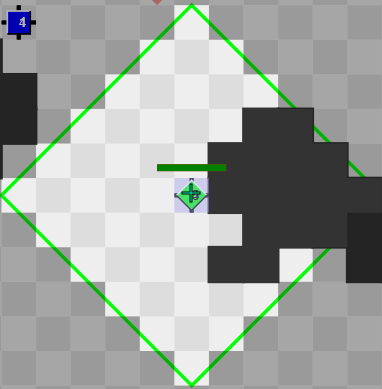
\includegraphics[width=150px]{bilder/agentensicht}
	\caption{Sicht des Agenten}
	\label{fig:agentensicht}
\end{figure}

Im ersten Schritt ermittelt der Agent einen möglichen Weg, wie er zu seinem Ziel gelangt. Hierfür wird der entsprechende Wegalgorithmus verwendet, welcher in Kapitel \textit{\ref{kap:wegfindung}} genauer erläutert wird. Sobald der Weg ermittelt wurde und bevor ein Schritt des Weges beschritten wird, prüft der Agent auf Aktionen, welche vorher ausgeführt werden müssen. Diese Aktionen können einen Rollenwechseln beinhalten, ungenutzte Blöcke fallen lassen, einen Block vom Dispenser anfordern oder einen Block aufnehmen, eine Aufgabe in der Endzone abgeben oder sich mit einem anderen Agenten verbinden. Diese Aktionen sind Momentaufnahmen, die der Agent ausführen muss, bevor er zu einem neuen Ziel geht. Wenn keine dieser Aktionen passt, wird der Agent den Weg zu seinem Ziel gehen. Hier kommt nochmals eine Entscheidungsmöglichkeit für den Agenten in Frage. Ist der nächste Schritt frei und ich kann den Weg gehen, dann geht er diesen. Sollte aber beispielsweise ein Block in der Richtung sein, in die der Agent gehen möchte, so muss er diesen zunächst zerstören. Wenn ein Agent in der Richtung steht, so wird ein Weg um diesen Agenten herum erstellt. In Abbildung \ref{fig:agentensicht} wäre der Weg in Richtung Westen durch einen Block gehindert, sodass er diesen zunächst zerstören muss, bevor er in diese Richtung gehen kann. 

Zusammengefasst muss der Agent in jedem Schritt entscheiden, ob es eine Aktion gibt, die gerade notwendig ist, wie einen Block aufzunehmen oder ob der Schritt, den er gehen möchte, möglich ist.  

\subsection{Synchronisation und Kommunikation}
Die Kommunikation der Agenten funktioniert, sobald sie sich in einer Gruppe befinden. Die Synchronisation der Gruppen ist in Kapitel \textit{\ref{kap:Gruppenbildung}} genauer beschrieben. Für die Kommunikation wurde eine Schnittstelle entwickelt, welche die Nachricht, den Senderagenten und den Empfängeragenten in einer Nachrichtenbox bereithält. Stehen zwei Agenten um einen Dispenser und beide möchten einen Block anfordern, so wird der Agent zunächst prüfen, ob eine Nachricht für ihn vorliegt. Ist dies nicht der Fall, untersucht der Agent, ob andere Agenten in der nähe des Dispensers stehen. Wenn die Prüfung erfolgreich ist, so wird er eine Nachricht an den Agenten senden und dieser wird dann warten, bis der Dispenser frei ist. Er selbst stellt eine Anfrage an den Dispenser und nimmt den Block dann auf.
